\documentclass[10pt]{article}
\usepackage[final]{graphicx}
\usepackage{amsfonts}

\usepackage{caption}
\usepackage{subcaption}

\topmargin-.5in
\textwidth6.6in
\textheight9in
\oddsidemargin0in

\def\ds{\displaystyle}
\def\d{\partial}

\begin{document}

\centerline{\large \bf Given a helical compression spring in a spring-mass-damper system, what are optimal springs?}

\vspace{.1truein}

\def\thefootnote{\arabic{footnote}}
\begin{center}
  Justin Krueger\footnote{Mathematics, Virginia Tech University},
  Alistair Bentley\footnote{Mathematics, Clemson University},
  Tianyu Qiu\footnote{Mathematics, University of Delaware},
  Saideep Nannapaneni\footnote{Civil \& Environmental Engineering,Vanderbilt University},
  Jiahua Jiang\footnote{Mathematics, University of Massachusetts Dartmouth },
  Tim Hodges\footnote{Mathematics, Colorado State University}
\end{center}

%\vspace{.1truein}

\begin{center}
Problem Presenters: Jordan Massad \footnote{Sandia National Laboratory},
Sean Webb \footnote{Sandia National Laboratory},
	Faculty Mentors: Ilse Ipsen\footnote{North Carolina State University},
	Ralph Smith\footnote{North Carolina State University}, 
\end{center}


\vspace{.3truein}
\centerline{\bf Abstract}




\begin{itemize}
\item Summarize the results presented in the report, and the contributions
of your research.




\item Readers should not have to look at the rest of the paper in order to 
understand the abstract.

\item Keep it short and to the point.
\end{itemize}

\section{Introduction}
%It should be written as much as possible in non-technical terms, so that a
%lay reader can understand the context and the contribution of the paper.

The use of mechanical switches in industry is a cornerstone of the modern world. Many mechanical switches can be designed to use a spring. This is useful because depending on the use of the switch, the spring can be optimized to for the function of the spring. 

For example, consider an acceleration switch in \ref{Acceleration Switch}. 

		\begin{figure}[h]
		 \begin{center}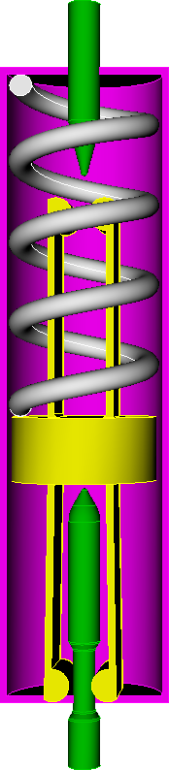
\includegraphics[scale=.2]{Acceleration_Switch.png}\end{center}
		 \caption{An example of an acceleration switch}
		 \label{Acceleration Switch}
		 
		 \end{figure}
\textbf{Describe problem, approach, and summarize contribution and results.}
This switch is used in high acceleration testing. The use is to only record information at crucial times of the test. For this reason when a certain force is exerted on the switch the pins at both ends will connect. When this happens we have a circuit that will enable data collection. It is important that the switch does not open too soon or too late otherwise the data collection will be too large or mean too little.This is just one example of a switch that we must know the best spring to make the performance maximal. For a more in depth look at this example look at \cite{IMSM2010}

Given that a switch may be used in a myriad of ways, it is important that one can find an optimal spring given after the use of the spring is known. This leads to an optimization problem. Even more this leads to an optimization problem that requires the flexibility to allow how a spring is determined to be optimal by an objective function and constraints. This does not consider the fabrication constraints that exist during manufacturing, but also needs to be considered as well. 

Given any constraint or objective function it will depend on a set of variables. This dependence will change when a constraint or objective function changes. In optimization we only wish to concern ourselves with the state variables that are allowed to change during optimization. For this reason, we construct a spring object that will hold all attributes of a spring and we can pull the relevant variables when it is determined what they are. 

In addition to this spring object, to reduce the uncertainty of the problem we conduct a sensitivity analysis of the objective function subject to the constraints and variables given. This allows the user to reduce the state variables if it is determined that the set of variables given has insensitive variables. 

A main contribution of this work is the framework to add constraints and objectives that may be unknown at the point of this paper. In parallel to this we have built a framework that is flexible enough to address the issue of unknown constraints and objectives. \textbf{ADD!}


\textbf{review history and existing literature}
Designing an optimal spring is not a new problem. In 2010 at the SAMSI IMSM workshop a team considered the design of an acceleration with enabled uncertainty. This approach lead to a paper \cite{IMSM2010}. This is not the only approach to uncertainty, in \cite{Reliability} probabilistic response surface methodology was implemented to investigate the complications of uncertainty in designing a spring. In addition to these types of approaches it is possible to narrow focus to a single parameter, in \cite{Robust} they focus on the spring stiffness. 

Our approach is not limited to an acceleration switch, instead it is but a special case of our approach. In \cite{Paredes} they attempt to design an optimal spring, with the introduction of a sizing tool. All references listed are informed to some extent by \cite{Wahl}. We do not focus on a set of parameters or attempt to fix the uncertainty of the spring design problem initially. We attempt to allow any possible construction of a spring optimization possible. 

This does not rule out if a construction is not physically or mathematically invalid. We will dispose of that case when we are unable to find a feasible point for optimization within our feasibility check. In summary, we need to allow any possible construction of a spring design problem, and adjust accordingly. 


\textbf{outline}
In this paper we will give a description of the springs of interest, helical compression springs. Next, the formulation of the problem, and the approach taken to the problem. Following will be a section on workflow with descriptions of each step in the workflow. Lastly, we will discuss a few case studies given the framework constructed and a summary with future work that can be worked on.



\begin{itemize}
\item Describe the problem you are trying to solve, the approach
you took, and summarize your contribution and results.

\item Review the history of this problem, and existing literature.

\item Give an outline of the rest of the paper.
\end{itemize}

\section{Helical Compression Springs}

Helical springs are a large class of springs sharing the common characteristic of a coiled appearance, see figure \ref{Spring}. 

		\begin{figure}[h]
		 \begin{center}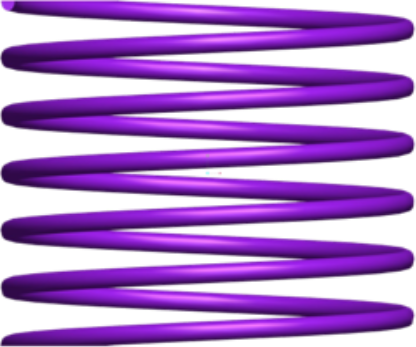
\includegraphics[scale=.2]{Spring.png}\end{center}
		 \caption{An example of a helical compression spring.}
		 \label{Spring}
		 
		 \end{figure}

Below is a list of a spring's key design parameters. We have added a few illustrations to keep straight some of the parameters. 		 
		\begin{figure}[h]
			\centering
			\begin{subfigure}{.5\textwidth}
				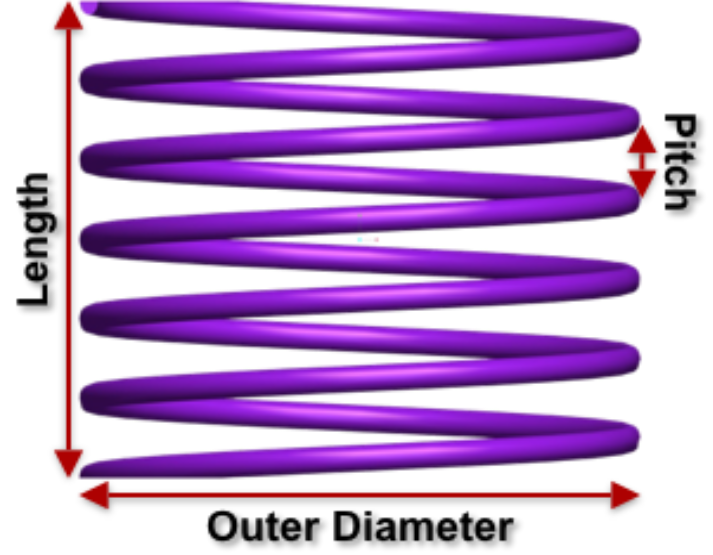
\includegraphics[scale=.2]{Spring_Description.png}
				\caption{Pitch, outer diameter, and length of a spring.}
				\label{Description1}
			\end{subfigure}%
			\begin{subfigure}{.5\textwidth}
				  \centering
		 		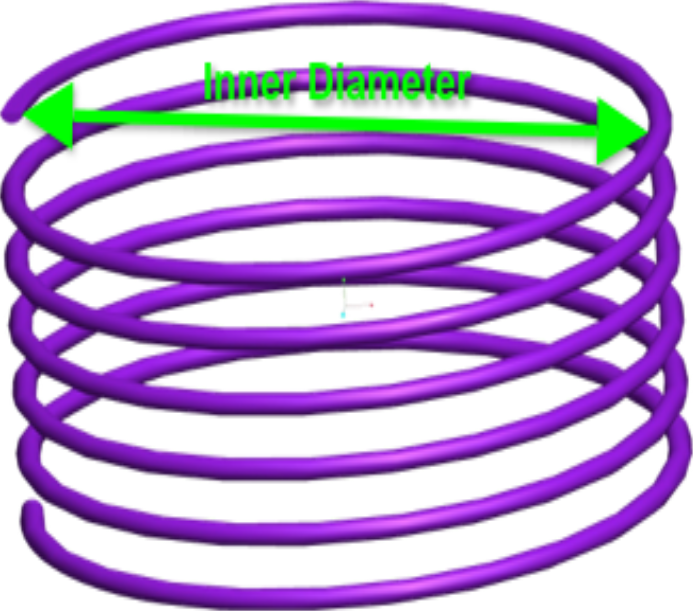
\includegraphics[scale=.2]{Spring_Description2.png}
				\caption{Inner diameter}
				  \label{Description2}
		  		
			\end{subfigure}
			 \label{Descriptions}
		  \caption{A few illustrations of a few of the parameters for a helical compression spring.}
		\end{figure}
		
		\begin{enumerate}
			\item Spring's inner diameter $d_{i}$, illustrated in figure \ref{Description2}.
			\item Spring's outer diameter $d_{o}$ illustrated in figure \ref{Description1}.
			\item Spring's wire diameter $d_{w}$.
			\item Total number of spring coils $N_{t}$.
			\item Active number of spring coils $N_{a}$, active coils are not touching any other coils, and is subject to the spring being closed or open. 
			\item Pitch $p$ illustrated in figure \ref{Description1}.
			\item Spring's free length $L_{free}$, this is the spring's length without any force applied. 
			
			\item Spring's solid length $L_{solid}$, this is the spring's length when all coils are compressed together.
			\item Spring's open length $L_{open}$, spring length at open position, open is beginning state.
			\item Spring's open length $L_{close}$, spring length at close position, close is the ending state.
			\item Spring's open length $L_{hard}$, the maximum a spring can compress for the application.
			\item Spring's open force $F_{open}$, this is the force on the spring in open position.
			
			
			\item Spring's shear modulus $G$, this is determined by the material of the spring.
			\item Spring's youngs modulus $E$, this is determined by the material of the spring.
			\item Spring's poisson ratio $\nu$, this is determined by the material of the spring.
		
		\end{enumerate}
		
		In addition to these parameters there are the following attributes that are empirical given some regime we care about.
		
			\begin{enumerate}
				\item Spring Rate, $$k = \frac{G}{8N_{a}}\frac{d_{w}^{4}}{(d_{i} + d_{w})^{3}}$$
				
				\item Spring Index, $$C = \frac{d_{i}}{d_{w}} + 1$$.
				
				\item Coil Binding Gap, $$g = \frac{L_{hard} - L_{solid}(d_{w},N_{a}; ec)}{N_{t} - 1}$$
		
				\item $$\frac{G(L_{free} - L_{hard})}{4 \pi N_{a} (ec)} \left[\frac{d_{w} (4d_{i}^{2} + 9.46d_{i} 
d_{w} + 3 d_{w}^{2})}{d_{i}(d_{i}+d_{w})^{3}}\right]< UTS$$ where UTS is the ultimate torsional stress.
		
				\item Diametral Expansion, $$d_{expand} = d_{w} + \sqrt{(d_{i} + d_{w})^{2} + 
				\frac{p_{closed}^{2} - d_{w}}{\pi^{2}}}$$
			\end{enumerate}
			
\section{The Problem} 

Design an algorithm that optimizes springs with interchangeable objectives and constraints. In addition, attempt to incorporate properties stress relaxation and creep into the available objectives and constraints. 

A list of possible constraints/objectives given in minimization form is below

\begin{enumerate}
\item $d_{i} < d_{i}^{max}$
\item $d_{i} < d_{o}$
\item $d_{i} + 2*d_{w} < d_{o}^{max}$
\item$d_{expand} - d_{0}^{max} < 0 $
\item$ \frac{G}{8N_{a}}\frac{d_{w}^{4}}{(d_{i} + d_{w})^{3}} - k_{max} \le 0 $
\item $\frac{d_{i}}{d_{w}} + 1 - C_{max}< 0$
\item $(L_{free} - L_{open})\frac{G}{8N_{a}}\frac{d_{w}^{4}}{(d_{i} + d_{w})^{3}} - F_{open} = 0 $
\item $\frac{L_{hard} - L_{solid}}{N_{t} - 1} + g_{min} \le  0$
\item$\frac{L_{free}}{d_{i} + d_{w}} - \pi \sqrt{\frac{2(2 \nu + 1)}{\nu + 2}}$
\item$-UTS + \frac{G(L_{free} - L_{hard})}{4 \pi N_{a} (ec)} \left[\frac{d_{w} (4d_{i}^{2} + 9.46d_{i} 
d_{w} + 3 d_{w}^{2})}{d_{i}(d_{i}+d_{w})^{3}}\right] < 0$
%\item Relaxation
\end{enumerate}	

\textbf{ADD RELAXATION HERE!}


In addition to these we should be able to minimize any attribute of the spring. 

In order to simplify the problem we have made some assumptions. First, we have assumed that constraints and objectives are all in terms of the number of total coils. This is to reduce the complexity of knowing if a constraint is dependent on the active number or total number of coils. These two numbers are dependent on the end conditions of the spring, whether it is open or closed at the end. For simplicity we also will consider all springs to be have a closed end condition. 

With these assumptions we simplify our constraints for pitch, $p$, solid length, $L_{solid}$, and the diametral expansion, $d_{expand}$. 

\textbf{JUSTIFY ASSUMPTIONS}

\section{The Problem}
\begin{itemize}
\item Give a precise technical description of your problem. 

\item State and justify all your assumptions. 

\item Define notation. 

\item Describe your data, how you collected them, their properties,
and whether you did 
anything to them (removed noise, filled in missing data, 
applied normalizations).
\end{itemize}

\section{The Approach}
\begin{itemize}
\item Present and justify your approach for solving the problem. 
\item Explain the advantages of your approach over existing ones.

\item Tell a story.
Don't just say: ``I did this, then I did this, and at last I did this''.
\end{itemize}

\section{Computational Experiments}
Give enough details so that readers can duplicate your experiments.

\begin{itemize}
\item Describe the precise purpose of the experiments, and what they 
are supposed to show.

\item Describe and justify your test data, and any assumptions you made to 
simplify the problem.

\item Describe the software you used, and the 
parameter values you selected.

\item 
For every figure, describe the meaning and units of the coordinate axes, 
and what is being plotted.

\item Describe the conclusions you can draw from your experiments
\end{itemize}

\section{Summary and Future Work}
\begin{itemize}
\item Briefly summarize your contributions, and their possible
impact on the field (but don't just repeat the abstract or introduction).
\item Identify the limitations of your approach.
\item Suggest improvements for future work.
\item Outline open problems.
\end{itemize}

\vfill\pagebreak

	
	\bibliographystyle{ieetr}

\bibliography{MyBib}



\end{document}

